\begin{example}[Advection 1D]
\label{ex:adv1D}
In $\Omega = [0, 1]$ we will solve the equation \eqref{eq:ex_advection}.
%\begin{equation}
%\pdiff{u}{t} + \fdiff{u}{x} = 0.
%\end{equation}
We use two initial conditions $u(0, x)$ to obtain two different solutions:
\begin{equation}
u_{smooth} = \begin{cases}
g(x),\quad &0.1 < x < .3\\
0, \quad &\text{elsewhere}
\end{cases},
\end{equation}
where
\begin{equation}
g(\xi) = \exp\left(\frac{1}{10(\xi - 0.2)^2 - 1}+ 1\right),
\end{equation}
and
\begin{equation}
u_{step} = \begin{cases}
\dfrac{1}{2},\quad &0.1 < x < .3\\
0, \quad &\text{elsewhere}
\end{cases}.
\end{equation}
The periodic boundary condition is prescribed at $x = 0$ and $x = 1$ --- this
results in the solution at time $t = 1$ to be the same as the initial condition,
i.e.
\begin{equation}
u(1, x) = u(0, x).
\end{equation}
%First we evaluate approximation of initial condition. As seen from figure
%\ref{fig:conv_0adv1D} the approximation corresponds to theoretical orders.
We then compare $u(1, x)$ with $u(0, x)$ to test the convergence, see Figure
\ref{fig:adv_conv_1D} and \ref{fig:adv_conv_1D_step}. For the smooth initial condition
the limiting increases the error of the solution due to artificial diffusion, higher order
methods are capable of counteracting this effect though. For the discontinuous initial
condition the limiting significantly improves the behavior of the method by removing 
oscillations and basically enabling use of high order methods, which suffer from them the 
most. This effect is illustrated in \Cref{fig:sol_adv1D}. The
resulting errors are still significant as the limiting introduces prominent
smoothing. Note that for both $u_{smooth}$ a $u_{step}$ with and without limiting the
convergence rate of the method is impacted by using the 3rd order TVD Runge-Kutta
time-stepping solver. This behavior is consistent with that reported by Krivodonova
\cite{Krivodonova2007}.

\end{example}
\begin{figure}[h!]
	\centering
	\begin{subfigure}{.5\textwidth}
		\centering
		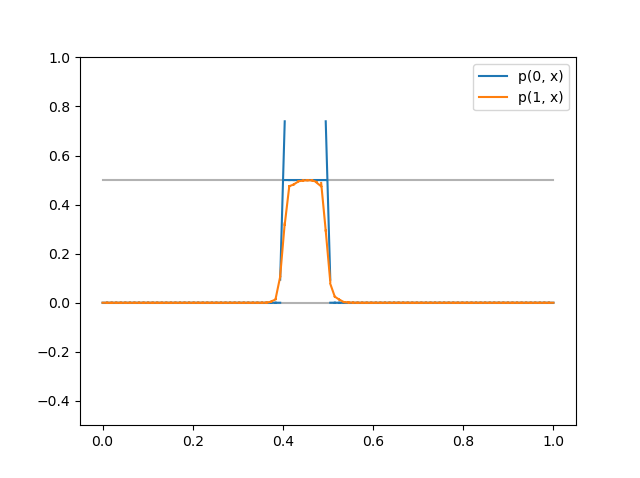
\includegraphics[width=\linewidth]{../figs/sols/adv1d-sol-o2h100-limit}
		\caption{Limit: True}
	\end{subfigure}%
	\begin{subfigure}{.5\textwidth}
		\centering
		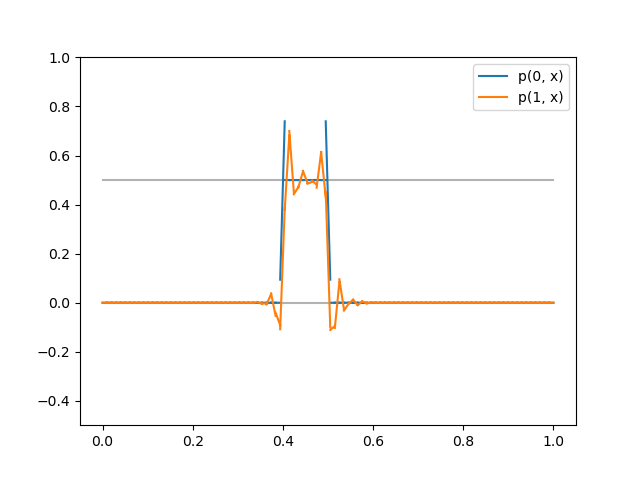
\includegraphics[width=\linewidth]{../figs/sols/adv1d-sol-o2h100-nolimit}
		\caption{Limit: False}
	\end{subfigure}
	\caption{\Cref{ex:adv1D}. Solution for $u_{step}$ for CFL coefficient $C_{CFL}=0.1$, 
	order $M = 4$, on uniform mesh with 100 elements.}
	\label{fig:sol_adv1D}
\end{figure}

\begin{figure}[p!]
	\centering
	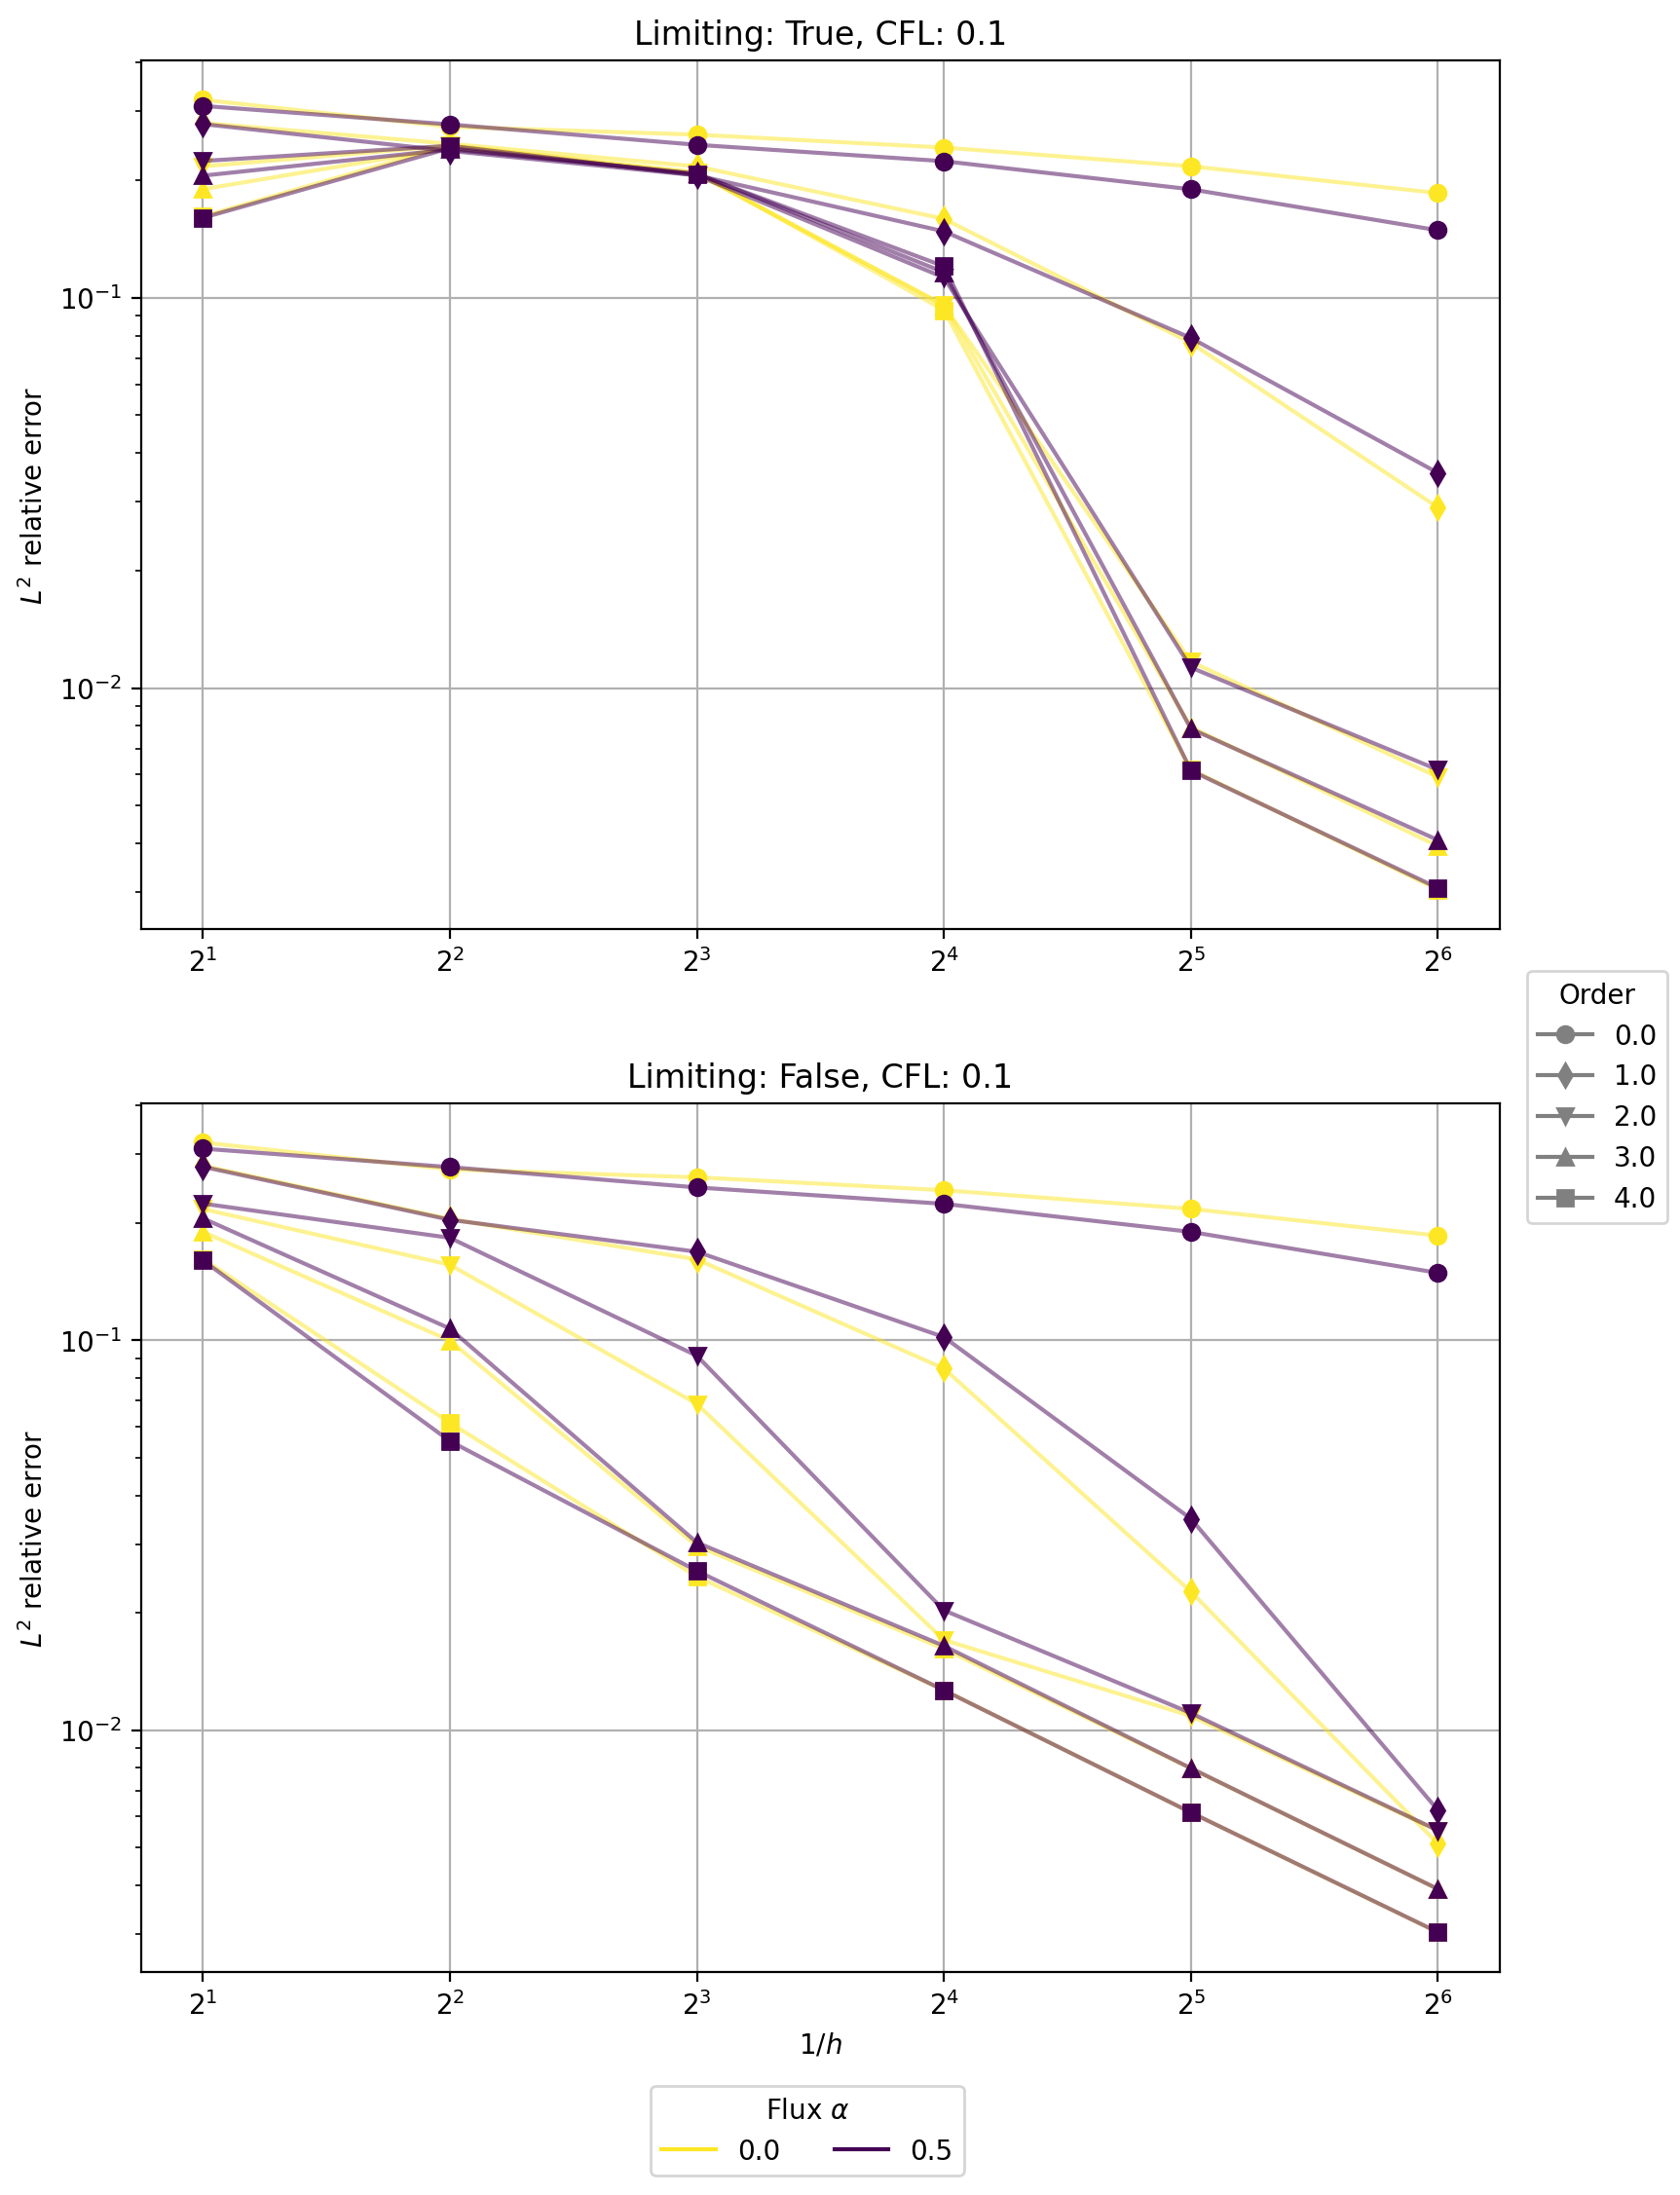
\includegraphics[width=1.1\textwidth]{../figs/parametric/advection_1D/advection_1D_smooth_reduced.png}
	\caption{\Cref{ex:adv1D}. Relative errors for smooth initial condition
		$u_{smooth}$.}
	\label{fig:adv_conv_1D}
\end{figure}


\begin{figure}[p!]
	\centering
	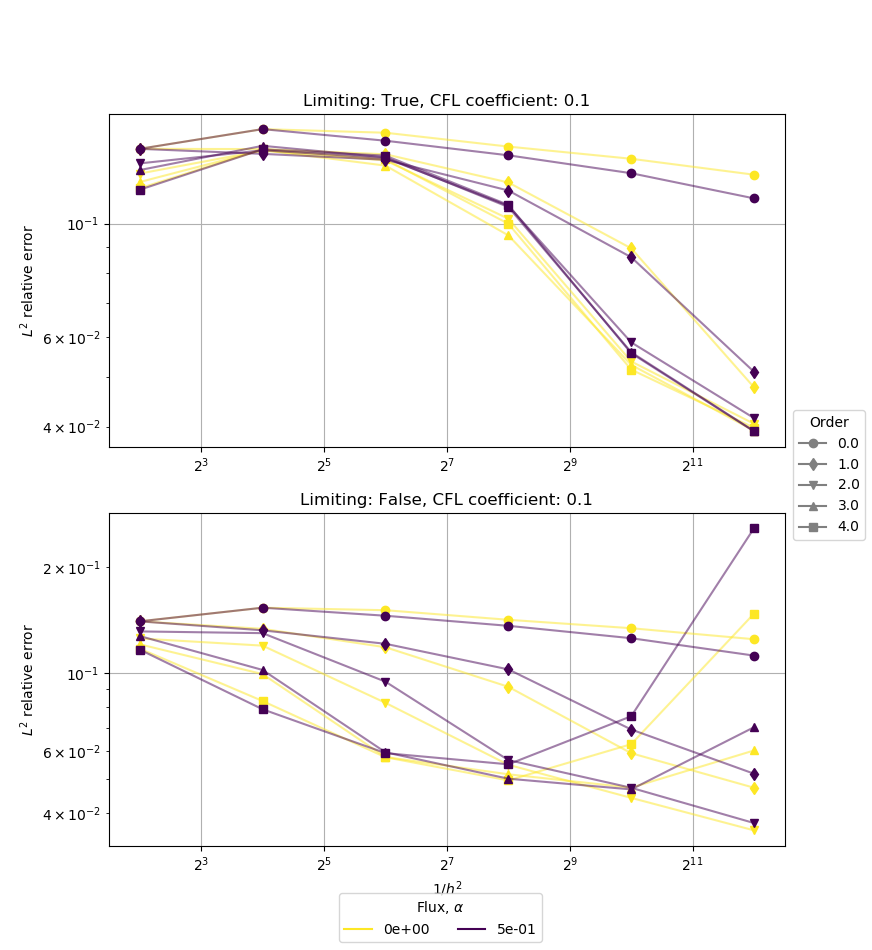
\includegraphics[width=1.1\textwidth]{../figs/parametric/advection_1D/advection_1D_step_reduced.png}
	\caption{\Cref{ex:adv1D}. Relative errors for discontinuous initial
	condition $u_{step}$.}
	\label{fig:adv_conv_1D_step}
\end{figure}
